%%This is the evaluation part, int includes the following parts.
% <1> Evaluation Metrics, explain the measurements chosen for this experiments
% <2> Test Platform in KNIME, the implementation, also the introduction of it
% <3> Test Cases Design, the parameters we want to compare, the cases
%   ==> synthetic data
%   ==> Real life data
%   ++ Data to test the property
This chapter presents an experimental evaluation of our techniques to repair model. At first, the evaluation measurements are defined. Next, we briefly introduce the test platform KNIME and ProM plugins tools for evaluation. In the following main part, the test on properties of our techniques is presented at the beginning. Then synthetic data is generated randomly to show the whole performance of our methods. At last, we conduct our experiments on real life data and also compare our techniques with other methods. The results show the ability of our techniques to repair model with high ranking according to defined measurements.
\section{Evaluation Measurements}
% First talk about our data and our model, then choose the confusion matrix as one measurements. But we should review the traditional measuremtns on process mining before introducing the confusion matrix. but we should also focus on the accuracy part and f-score.
We evaluate our techniques based on the quality of repaired models with respect to the given event logs. In process mining, there are four quality dimensions generally used to compare the process models with event logs. 
\begin{itemize}
	\item \emph{fitness.} It quantifies the extent of a model to reproduce the traces recorded in an event log which is used to build the model. Alignment-based fitness computation aligns as many events from trace with the model execution as possible.  
	\item \emph{precision.} It assesses the extent how the discovered model limits the completely unrelated behavior that doesn't show in the event log. 
	\item \emph{generalization.} It addresses the over-fitting problem when a model strictly matches to only seen behavior but is unable to generalize the example behavior seen in the event log. 
	\item \emph{simplicity.} This dimension captures the model complexity. According to Occam's razor principle, the model should be as simple as possible.
\end{itemize}
% How to come to confusion matrix?? 
The four traditional quality criteria are proposed in semi-positive environment where only positive instances are available. Therefore, when it comes to the model performance, where negative instances are also possible. The measurement metrics should be adjusted. The repair techniques in this thesis are based on the labeled data and the repaired model can be seen as a binary prediction model where the positive instances are supported while the negative ones are rejected. The model evaluation becomes a classification evaluation. 
% Describe its features and some derived measurements. 
Confusion matrix has a long history to evaluate the performance of a  classification model. %A confusion matrix for the repaired model is a table with two rows and two columns to describe the actual observed behavior and model execution. 
A confusion matrix is a table with columns to describe the prediction model and rows for actual classification on data.  The repaired model can be seen a binary classifier and produces four outcomes- true positive, true negative, false positive and false negative shown in the Table \ref{tab:cm}.
\begin{itemize}
	\item True Positive(TP): The execution allowed by the process model has an positive performance outcome.
	\item True Negative(TN): The negative instance is also blocked by the process model.
	\item False Positive(FP): The execution allowed by the process model has an negative performance outcome.
	\item False Negative(FN):The negative instance is enabled by the process model.
\end{itemize} 
% confusion matrix
\begin{table}[]
	\caption{Confusion Matrix}
	\label{tab:cm}
	\begin{tabular}{ll|c|c|}
		\cline{3-4}
		&                   & \multicolumn{2}{c|}{repaired model}                                               \\ \cline{2-4} 
		\multicolumn{1}{l|}{}                                                                         &                   & \multicolumn{1}{l|}{allowed behavior} & \multicolumn{1}{l|}{not allowed behavior} \\ \hline
		\multicolumn{1}{|l|}{\multirow{2}{*}{\begin{tabular}[c]{@{}l@{}}actual \\ data\end{tabular}}} & positive instance & TP                                    & FN                                        \\ \cline{2-4} 
		\multicolumn{1}{|l|}{}                                                                        & negative instance & FP                                    & TN                                        \\ \hline
	\end{tabular}
\end{table}
Various measurements can be derived from confusion matrix. According to our model, we choose the following ones as the potential measurements. 
\begin{itemize}
	\item recall. It represents the true positive rate and is calculated as the number of correct positive predictions divided by the total number of positives.
	\[Recall = \frac{TP}{TP + FP}\]
	\item precision. It describes the ability of the repaired model to produce positive instances.
	\[Precision = \frac{TP}{TP + FN }\]
	\item specificity. In opposite with recall, it measures the true negative rate.
	\[Specificity = \frac{TN}{TN + FP}\]
	\item accuracy. It is the proportion of true result among the total number. It  measures in our case how well a model correctly allows the positive instances or disallows the negative instances.
	\[Accuracy = \frac{TP+TN}{TP+TN+FP+FN}\]
	\item F-score is is the harmonic mean of precision and recall.
	\[F_1 = \frac{2*Recall*Precision}{Precision + Recall}\]
\end{itemize}
After experiments we can see that accuracy gaine more weights than precision.


Generally, there is a trade-off between the quality criteria. So the measurements are only used to compare specific aspects of our techniques.
\section{Experiment Platform}
Data simulation part
Try to automatize and standardize experiments, in order to make this experiments more effective, and easier to repeat. So KNIME is selected as one of the test platform to perform tasks. Also, some existing evaluation plugins in ProM are used to evaluate on the other aspects.

\subsection{PLG}
Process Log Generator(PLG) is designed to generate random business processes models and event logs according by setting the complexity parameters. Complexity parameters for model generation in PLG include the maximum number of branches for activities relation parallel, or exclusive choices,  maximum depth of nested pattern, the weights on relations, and so on. The parameters to generate an event log are, for example, number of traces, and noise on the workflow or missing rate of trace heads. 

In this experiment, process models in Petri net are randomly created by inputting simple, normal and complex parameters settings. Event logs are also simulated according to different complexity level. The setting details is in Table??. 
\subsection{KNIME}
KNIME Analytics Platform is open source software in Java to help researcher analyze data by integration of multiple modules for loading, process and transformation and machine learning algorithms. Researcher can achieve their goals by creating visual workflows composed of modules with an intuitive, drag and drop style graphical interface, rather than focusing on any particular application area. 
The reason to choose KNIME as our experiment platform is that KNIME supports automation of test workflow which is more efficient.  
However, to conduct experiments, the related modules of our algorithm have to be integrated into KNIME, which requires additional development effort. At end, process mining modules like event logs, basic process models reader and writer, basic logs manipulators, classic discovery algorithms, and model repair are imported into KNIME.
\subsection{ProM Evaluation Plugins}
Here we discuss the plugins to test other aspects of our methods. 
\section{Experiment Result}
\subsection{Test On Property}
In this experiment, we aim to answer the questions: 1) How do our techniques incorporate the existing model, positive and negative information to repair model? 2) How do the techniques overcome the shortcomings of current state-of-the-art repair techniques?
To answer the first question, we applied the repaired techniques on event logs with different relations of activities, such as sequence, parallel and loop, exclusive choice and investigated the effect from the existing model, positive and negative instances on the repaired model, by adjusting the corresponding weights. For the second question, we describe the situations where our techniques overcome the defects of other repair techniques and explain the reasons behind it. 
\subsubsection{Test On Sequence}
This part is used to show the effect of our techniques on the sequence relation of activities. Given a fixed model in Petri net with sequence relation, a set of event logs with different deviations are used to test if our repair techniques work properly.
% The experiments go in this way, given a model, we changed them by looking all the information and then giving them effect on them relation, should we put all experiments, let's do it, later we can modify it.
\begin{figure}
	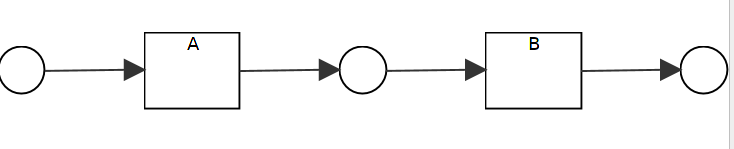
\includegraphics[width=0.9\textwidth]{figures/evaluation/model_01_sequence.png}
	\caption{Model M1 with sequence relation}
	\label{fig:sequence-M1}
\end{figure} 
\begin{itemize}
	\item \emph{Experiment 1} delete activity from sequence relation \\
	
	\emph{Event Log: }
	\begin{align*}
	Positive:& {<a>}^{50} \\
	Negative:& {<a, b>}^{50}
	\end{align*}
	% repair result from them, one is the repaired model, second is the plot lines with weight changes
	\emph{Repair Result}
	
	
	\item 
\end{itemize}
\subsubsection{Test On Parallel}
This part shows how the parallel relation of activities is affected by the weights for the existing model, positive and negative instances.
%% Here we need to paste the picture and its analysis together..create a table to remark the name and its analysis in doc.

\subsubsection{Test On Loop}
This part investigated our repair method on activities with loop relation.

\subsubsection{Test On Exclusive Choice}
This part displays the changes of exclusive choices relation in the model under the different control weights.

\subsection{Comparison To Other Techniques}
This section represents some situations where current repair techniques can't handle properly, while our algorithm gives out an improved repaired model. 

Situation 1, unfit part!! added subprocess are too much!! Where the addition of subprocesses and loops are allowed, while the structure changes are impossible, 
Fahrland's method applies the extension strategy to repair model by adding subprocesses and loops in the procedure. It introduces unseen behavior into the model. However, if the behaviors which are already in the model is unlikely to be removed from the model. One simple example is shown in the following part. 

Dee's method is based on Fahrland's method. Deviations are calculated at first and used to build subprocesses for model repair. However, before building subprocesses, it classifies the deviations into positive and negative ones with consideration of trace performance. Only positive deviations are applied to repair model. Different to Fahrland's method, it improves the repaired model performance by limiting the introduced subprocesses. Still, it can't get rid of the defect mentioned before. 

Situation 2, For fitted data in the model, can not recognize them!! where overlapped data noise can not be recognized, trace variant with more negative effect is treated as positive and kept in the model, which we should delete them.   
% Here we want to give an example of the overlapped data, compared to IM rediscoverty, easy.. But for Dees' method, firstly, they have labeled data; The analyzed the deviations of them, but when one deviation dominates, then the tree can not see the others. Some data are ignored..

Situation 3, with long-term dependency!! fitted part or new added part!! none of the current techniques can handle this problem yet.
Simple examples listed, but will this repeat the last section?? 


% Conclusion part
For one exclusive choices, 
but with long-term dependency detected and added in the model, precision and accuracy increase, since model with long-term dependency blocks the negative information by adding transitions and places to limit activity selection. 
\subsection{Test On Synthetic Data}
Those synthetic data is generated randomly by using the simulation tool plg %should cite it and to the end, or we just mentioned it before in the preparation parts. 
\subsection{Test On Real life Data}
